%\vspace{-0.1in}
\section{\sysname{} for Clos Topology}
\label{sec:specific}

\begin{figure}[t]
		\centering
		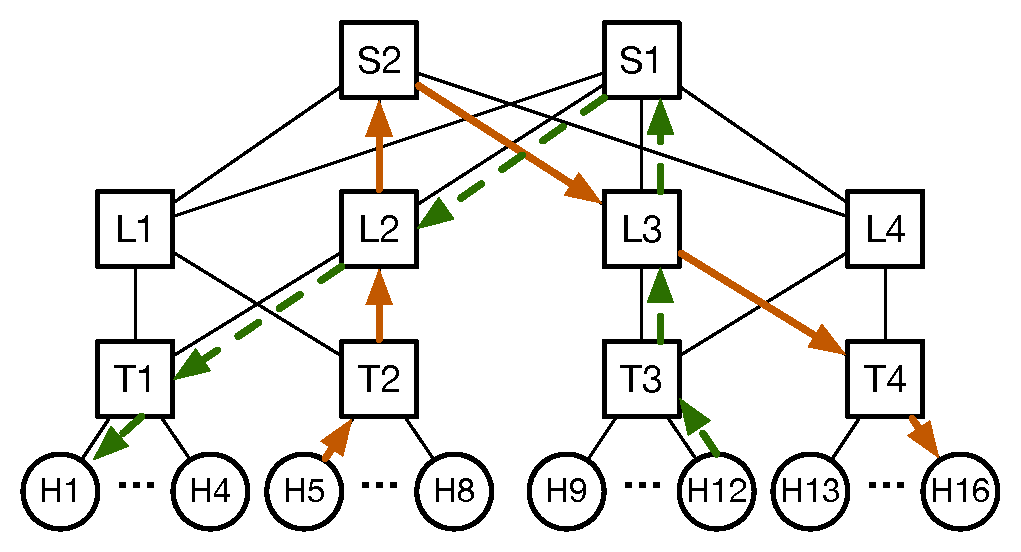
\includegraphics[width=0.4\textwidth] {figs/updown_paths}
		\caption{Clos topology with two flows following up-down routes}
		\label{fig:basic_clos}
\end{figure}

While \sysname{} works for any topology, we first describe the core ideas using
the popular Clos network topology. 

\subsection {Preliminaries}

\para{Expected Lossless routes:} This is a set of packet paths that network
operators requires to be lossless. For example, in a Clos network, the
operator may want that all up-down paths are lossless. In the rest of the
section, we refer to these routes simply as lossless routes. 

\para{Lossless class:} A lossless class is a service that we provide for
applications. The network guarantees that packets in a lossless class will
not be dropped due to buffer overflow as long as they traverse lossless paths.

\para{Tag:} Tag is a small integer assigned / associated with a packet. The tag
is embedded in a packet. A packet belonging to one lossless class may change its
tag value, which means that a lossless class may have multiple tag values.

\para{Switch model:} For ease of discussion, we use the following simplified
switch model\footnote{See \S\ref{sec:implementation} for full implementation
details.} in this section.  A switch has multiple ports. Each port has upto 7
lossless queues associated with it, and one lossy queue\footnote{Typically,
there is just one shared buffer and ``queues'' are just ``views'' of this shared
buffer.} The queue number corresponds to the PFC priority.  Switch classifies
arriving packets into queues based on {\em tags}.  Typically, each tag maps to a
single priority value. If a tag does not match any priority value, the packet is
added to a lossy queue. Before forwarding a packet, the switch can rewrite the
tag according to user-specified rules.

We now describe the core idea behind \sysname{}.

\subsection{Tagging on bounce}
\label{subsec:tag}

\begin{figure}[t]
	\centering
	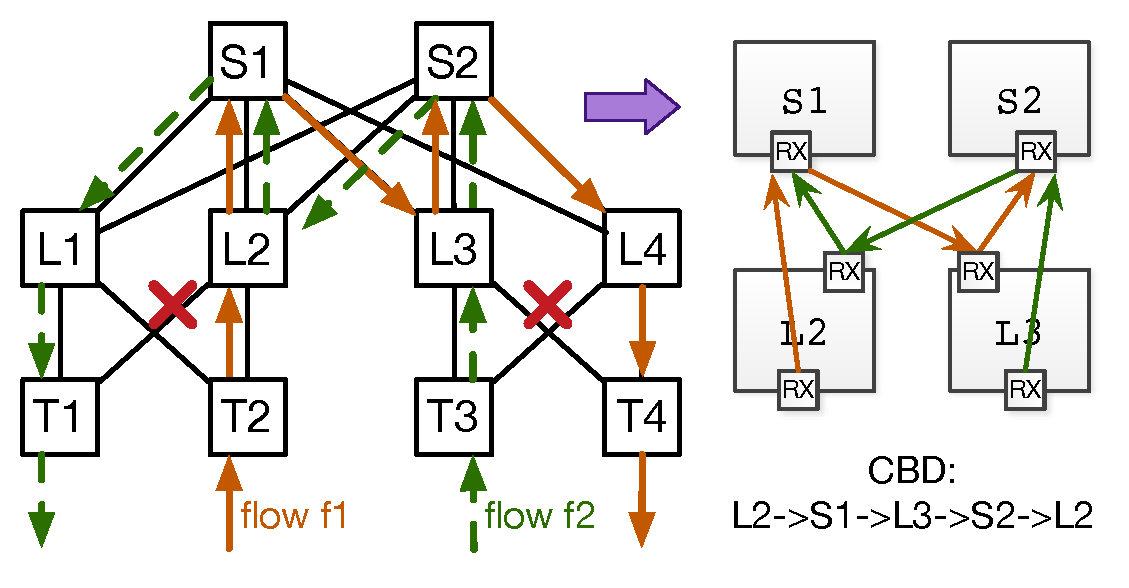
\includegraphics[width=0.5\textwidth] {figs/cbd_a}
	\caption{1-bounce path creates CBD}
	\label{fig:clos_1_bounce}
\end{figure}

Recall Figure~\ref{fig:basic_clos}. Both the green and blue flows follow up-down
routing and there is no deadlock. 

Now, let's assume that as shown in Figure~\ref{fig:clos_1_bounce}, two
links fail, which forces both flows to deviate from up-down paths ($L2$ to
$S1$ for green flow, $L3$ to $S2$ for blue flow). We call these paths 1-bounce
paths, as the path violates the up-down rule once. As shown, this can lead to
CBD, and hence may cause deadlock.

One way to avoid such CBD is to put any packets that have deviated from the
up-down routes in a lossy queue.  Being assigned to lossy queue means that such
packets will not trigger PFC. Since the basic up-down paths are deadlock free,
and the bounced packets do not trigger PFC, the network will stay deadlock free
even if packets bounce.

We stress that being assigned to lossy queue does not mean that the packets are
immediately (or ever) dropped -- they are dropped {\em only if} they arrive at a
queue that is full. The only thing we need is that these packets not trigger
PFC.

Thus, if each switch can detect that an arriving packet has deviated (sometime
in past) from the up-down path, it can put it in lossy queue, and there will be
no deadlock.

Note that this solution requires no changes to existing routing protocol.  But
how can a switch determine whether the packet has bounced, using just local
information, in presence of dynamic routing?

Consider the green flow in Figure~\ref{fig:clos_1_bounce}.  We want switch $S1$,
the first switch after bounce, to detect the bounce and put the packet in a
lossy queue. 

One way for $S1$ (and any other switch afterwards) to recognize a bounced packet
is by TTL - a bounced packet will have ``lower than expected'' TTL. However, TTL
values are set by end hosts~\footnote{TTL has other disadvantages as well,
see \S\ref{subsec:caveats}}, so a more controllable way is for the switch $L2$
to provide this information.  In normal ``up-down'' routing, $L2$ would never
forward a packet that arrived from $S2$ to $S1$. So, if $L2$ ``tags'' packets
that have arrived from $S2$ that it is forwarding to $S1$, then $S1$, {\em and
all other switches along the path after $S1$} know that the packet has deviated
from the up-down path.

Note that $L2$ needs only local information to do the tagging. We can initially
assign a $NoBounce$ tag to every packet. $L2$ then simply needs to check ingress
and egress port for each packet: it changes the tag from $NoBounce$ to $Bounced$
if a packet arriving from ingress port connected to $S2$ exits on egress port
connected to $S1$.  It is easy to see that these rules can be pre-computed since
we know the topology, and the set of routes that we want to be ``lossless''
(i.e. the up-down routes). 

This, in essence, is the core idea behind \sysname{} -- leveraging the knowledge of
topology, and the paths that need to be lossless, we can create a system of tags
and {\em static} rules that manipulate these tags to ensure that there will not
be CBD, despite dynamic routing.

Of course, this basic idea is not enough. First of all, packets may bounce not
just from the spine layer, but at any layer. Second, recall from
\S\ref{sec:reroute} that ``bounces'' are a fact of life in data center networks.
The operator may not want to put packets that have suffered just a single bounce
into a lossy queue -- we may want to wait until the packet has bounced more than
once before assigning it to a lossless queue. Third, we must ensure that we
don't end up using more lossless queues than the switch can support. To this
end, we show how to combine tags.

\begin{figure}[t]
	\centering
	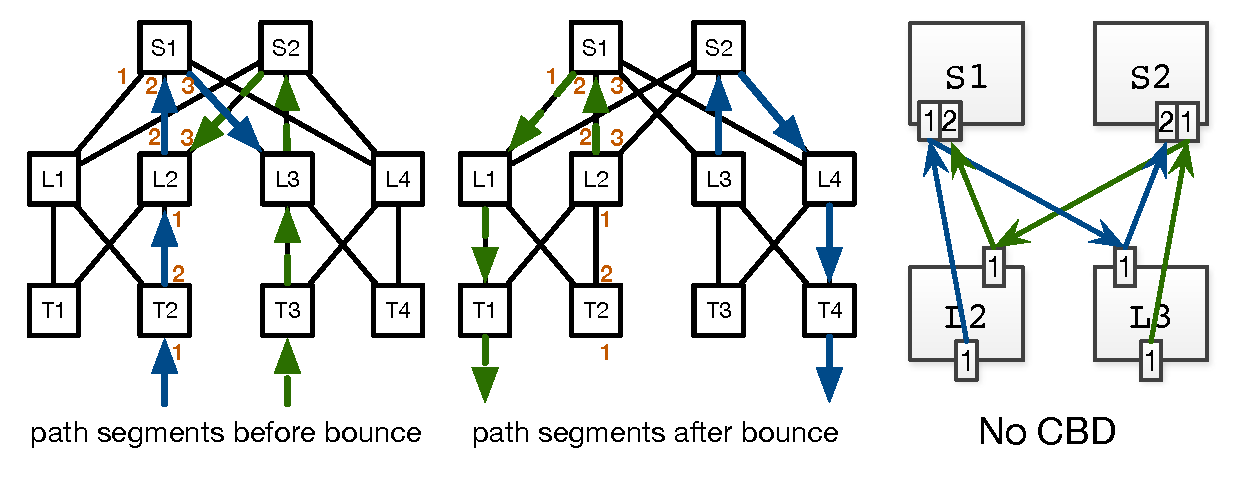
\includegraphics[width=0.5\textwidth] {figs/cbd_b}
	\caption{\sysname{} eliminates CBD by separating before-and-after bounce path segments}
	\label{fig:clos_tagger}
\end{figure}

\subsection{Reducing the number of lossless queues}
\label{subsec:combine}

In Clos network as shown in Figure~\ref{fig:basic_clos}, packets can
bounce at any $L$ layer, or called Leaf, switches. In addition, packets can also
bounce at any $T$ layer, or ToR switches. Do we need to assign a distinct tag
and a corresponding priority queue for each bouncing point? 

Again, we leverage our knowledge of Clos topology and routing. Consider a packet
that bounces twice. The path between the first bounce and the second bounce is a
normal up-down path. Therefore, these path segments do not have CBD even if we
combine them into a single priority queue. We can use a single tag to represent
these segments altogether, and map the tag to a globally unique priority queue.

This completes the design of \sysname{} for Clos topology.  We first tag all
packets following the normal ``up-down'' routing input with tag value of 1. All
switches put these packets into first lossless queue. Then we configure all ToR
and Leaf switches such that every time they see a packet coming down and then
going up (therefore, bouncing) for any reasons, they increase the tag by one.
Assuming there are $k$ available lossless queues, all switches put packets with
tag $i$ to $i^{th}$ lossless queues. This means packets with up to $k-1$ bounces
are all lossless. If a packet bounces more than $k-1$ times, it will carry a tag
larger than $k$. All switches will put such packets into a lossy queue.
Pseudocode of the algorithm, using notation developed in \S\ref{sec:generic}, is
shown in Appendix~\ref{sec:clos_optimal}.

Figure~\ref{fig:clos_tagger} illustrates the tagging algorithm in
action.  Packets, when travelling on path segments before bounce carry a tag
value of 1, and the tag is set to 2 after the bounce. This ensures that the
packets are queued in separate lossless queues, and thus there is no CBD. In
other words, we show a system for $k=2$. The lossy queue for packets that bounce
more than once is omitted for clarity. 

This design satisfies all three challenges described in
\S\ref{sec:challenges}. We do not change the routing protocol. We work with
existing hardware. We deal with dynamic changes to routes, and we do not exceed
the number of available lossless queues.

\subsection {Deadlock freedom and optimality}
\label{subsec:specific_deadlock_free}

We now provide brief proof sketches to prove that the above algorithm is
deadlock free, and optimal in terms of number of lossless priorities used.

\begin{figure}[t]
	%\vspace{-0.1in}
	\centering
	
	\subfloat[short for lof][CBD across subspaces.] {
		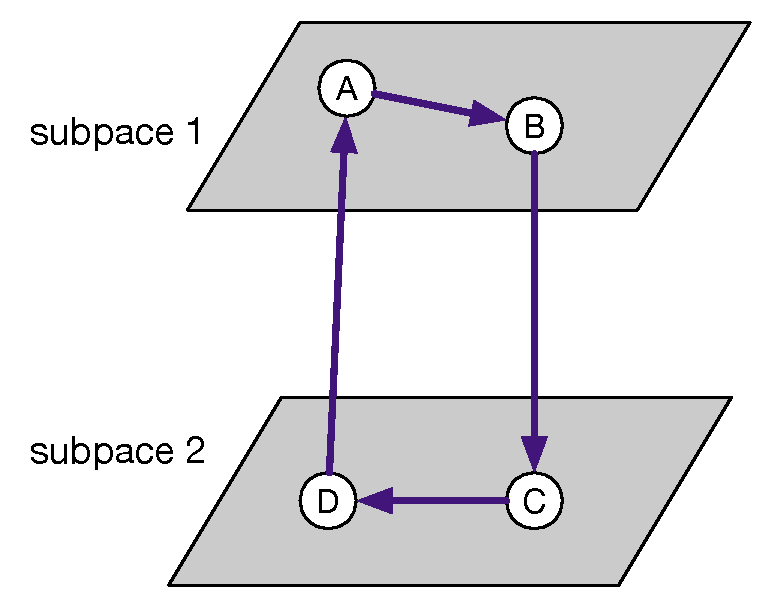
\includegraphics[width=0.24\textwidth] {figs/subspace_a}
	}
	\subfloat[short for lof][DAG across subspaces.]{
		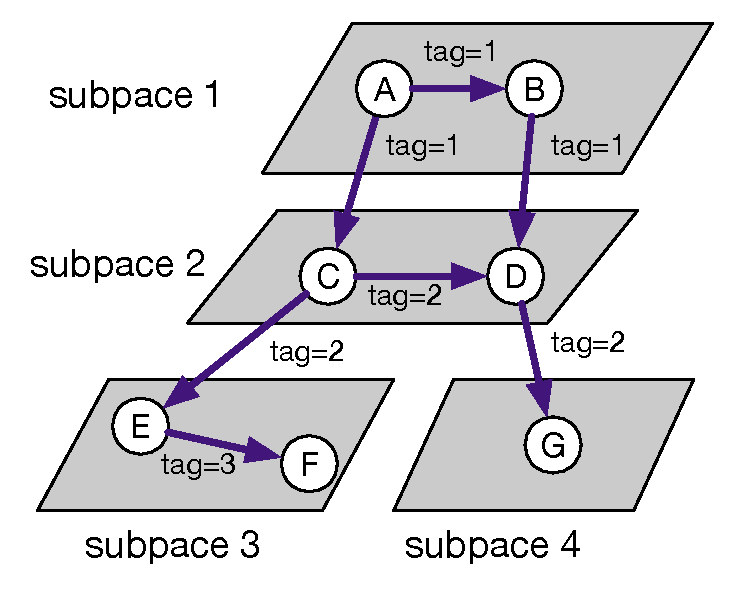
\includegraphics[width=0.26\textwidth] {figs/subspace_b}
	}
	
	\caption{DAG across subspaces ensure deadlock-free priority transition.}\label{fig:subspace}
\end{figure}

\para{\sysname{} is deadlock-free for Clos networks:} \sysname{} has two
important properties. First, for any given tag and its corresponding priority
queue, there is no CBD because each tag only has a set of ``up-down'' routing
paths.  Second, every time the tag changes, it changes monotonically. This means
that the packet is going unidirectionally in a DAG of priority queues. This is
important because otherwise CBD may still happen across subspaces
(Figure~\ref{fig:subspace}).  We conclude that no CBD can form either within a
tag or across different tags.  The network is deadlock-free since CBD is a
necessary condition of deadlock~\cite{our_hotnets_paper}.  A formal proof, which
also applies for generic topology, is given in \S\ref{sec:generic}. 

\para{\sysname{} is optimal in terms of lossless priorities used:} We show that
to make all $k-1$ bounces paths lossless and deadlock-free, at least $k$
lossless priorities are required. We use contradiction.  Assume there exists a
system with only $k-1$ lossless priorities. Consider a flow that loops between
$T1$ and $L1$ for $k$ times, which means bounces $k-1$ times at $T1$. With
Pigeonhole principle, we know that at least two times during the looping, the
packet must have the same lossless priority. This is already sufficient to cause
a deadlock~\cite{our_hotnets_paper}. Contradiction.

\subsection {Summary}

We showed that given a Clos topology and a set of routes (up-down, plus
upto $k-1$ ``bounces'') that should be lossless, we can generate a system of
tags and associated rules that ensure that packets are correctly classified
into $k$ lossless queues to ensure that there is no deadlock.   This system can
be implemented with existing hardware, without requiring any changes to the
routing protocol. We also showed that this system is optimal, in the sense that
we cannot prevent deadlock with fewer lossless queues.

We now show how to generalize \sysname{} for any topology.
